\documentclass[11pt,aspectratio=169]{beamer}

\usetheme{metropolis}
\usepackage{amsmath,amssymb,amsfonts,bm,mathtools}
\usepackage{booktabs,multirow,array}
\usepackage{tikz}
\usetikzlibrary{arrows.meta,positioning,calc,fit,shapes.geometric,decorations.pathreplacing}
\usepackage{graphicx}
\usepackage{xcolor}

% Match metropolis palette with a slight tweak
\definecolor{cb}{HTML}{1f77b4}\definecolor{cr}{HTML}{d62728}
\definecolor{cg}{HTML}{2ca02c}\definecolor{cy}{HTML}{ff9f00}

% Math shorthands
\newcommand{\R}{\mathbb{R}}
\newcommand{\E}{\mathbb{E}}
\newcommand{\Prb}{\mathbb{P}}
\newcommand{\argmax}{\operatorname*{arg\,max}}
\newcommand{\bel}{\mathbf{b}}
\newcommand{\state}{\mathcal{S}}
\renewcommand{\action}{\mathcal{A}}
\newcommand{\Obs}{\mathcal{O}}

\tikzset{
  chance/.style={ellipse,draw,fill=cb!15,minimum width=14mm,minimum height=10mm,thick,inner sep=1pt,font=\small},
  decision/.style={rectangle,draw,fill=cg!18,minimum width=14mm,minimum height=10mm,thick,rounded corners=1pt,inner sep=2pt,font=\small},
  utility/.style={diamond,draw,fill=cy!25,minimum width=14mm,minimum height=10mm,thick,inner sep=-2pt,aspect=1.4,font=\small},
  state/.style={circle,draw,fill=cb!15,minimum size=12mm,thick,inner sep=1pt,font=\small\bfseries},
}

\title{Regime-Switching Asset Allocation via a POMDP}
\subtitle{Type: New Application}
\author{Dario Blanco Morales \and Even Hogberget \\ Kyle D. Ledda-Lewaren \and Taka Khoo}
\institute{\footnotesize ENGS 177, Decision Making Under Uncertainty \\ \footnotesize Thayer School of Engineering, Dartmouth College}
\date{\footnotesize May 2026}

\begin{document}

%-------- Title --------
\begin{frame}\titlepage\end{frame}

%-------- Slide 1: Motivation --------
\begin{frame}{The problem: regimes break static allocation}
\textbf{The 60/40 portfolio lost $\sim$17\% in 2022.}
\smallskip

A static allocation assumes stable joint return moments. Markets violate
this in two ways:
\begin{itemize}
  \item \textbf{Conditional heteroskedasticity:} long quiet periods broken by short crises.
  \item \textbf{Stress correlation:} stocks and bonds sell off together when it hurts most.
\end{itemize}

\medskip
\textbf{Question.} Can a decision-theoretic regime overlay, a POMDP solved
end-to-end on macroeconomic observables, beat a static benchmark after
realistic frictions?
\end{frame}

%-------- Slide 2: Why POMDP (one decision/lecture tree) --------
\begin{frame}{Why POMDP, not a tree, ID, or MDP}
\begin{tabular}{ll}
\toprule
\textbf{Naive choice} & \textbf{Why it fails here} \\
\midrule
Decision tree & Tree explodes with horizon; no shared state. \\
Influence diagram & Same blow-up; not natural for repeated rebalance. \\
Fully-observable MDP & Requires knowing the regime, but it is \emph{latent}. \\
\textcolor{cb}{\textbf{POMDP}} & \textcolor{cb}{Hidden state, Bayesian belief, QMDP for tractable control.} \\
\bottomrule
\end{tabular}

\medskip
\textbf{Tools assembled:} Bayesian forward filter; Markov chain over regimes;
infinite-horizon Bellman recursion solved by value iteration and exact
policy iteration; structural results for monotone policies.
\end{frame}

%-------- Slide 3: POMDP tuple --------
\begin{frame}{POMDP tuple, written once and reused}
\small
\begin{description}[itemsep=2pt,topsep=2pt]
  \item[$\mathcal{T}$] $=\{0,1,2,\dots\}$, monthly epochs.
  \item[$\state$] $=\{s_1,\dots,s_K\}$ latent regimes ($K=2,3,4$).
  \item[$\action$] $=\{(0/100),(20/80),\dots,(100/0)\}$ discrete portfolio grid.
  \item[$T(s'\mid s)$] HMM transition matrix; \alert{action-independent} (regimes are exogenous).
  \item[$O(\mathbf{o}\mid s)$] Gaussian emission on $\mathbf{o}=(\mathrm{VIX},\mathrm{term\ spread})$.
  \item[$R(s,\mathbf{a})$] $=\E[\,U(\mathbf{a}^\top\mathbf{r})\mid s\,]-c\lVert\mathbf{a}-\mathbf{a}_{\rm prev}\rVert_1$, CRRA utility.
  \item[$\lambda=0.95$] monthly discount.
\end{description}
\medskip
\textbf{Belief update (Bayesian filter):}
$\bel_t(s')\propto O(\mathbf{o}_t\mid s')\!\sum_s T(s'\mid s)\,\bel_{t-1}(s).$
\end{frame}

%-------- Slide 4: Pipeline diagram (TikZ) --------
\begin{frame}{Pipeline}
\centering
\scalebox{0.85}{
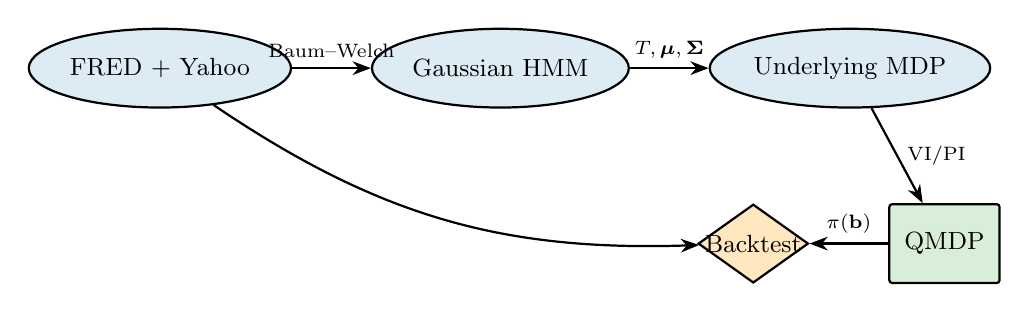
\begin{tikzpicture}[node distance=6mm and 10mm,>=Stealth]
  \node[chance] (data) {FRED + Yahoo};
  \node[chance,right=of data] (hmm) {Gaussian HMM};
  \node[chance,right=of hmm] (mdp) {Underlying MDP};
  \node[decision,below=12mm of mdp,xshift=12mm] (qmdp) {QMDP};
  \node[utility,left=of qmdp] (back) {Backtest};
  \draw[->,thick] (data)--(hmm) node[midway,above,font=\scriptsize]{Baum--Welch};
  \draw[->,thick] (hmm)--(mdp) node[midway,above,font=\scriptsize]{$T,\bm{\mu},\bm{\Sigma}$};
  \draw[->,thick] (mdp)--(qmdp) node[midway,right,font=\scriptsize]{VI/PI};
  \draw[->,thick] (qmdp)--(back) node[midway,above,font=\scriptsize]{$\pi(\bel)$};
  \draw[->,thick] (data) to[bend right=18] (back);
\end{tikzpicture}}
\medskip

\begin{itemize}
  \item Raw observations $\to$ HMM emissions and transitions.
  \item HMM transition matrix becomes the MDP's $T$. Reward built by MC.
  \item VI and PI cross-checked. QMDP folds belief into $Q^\ast$.
  \item Backtest is a walk-forward filter+act loop on real history.
\end{itemize}
\end{frame}

%-------- Slide 5: Regime calibration --------
\begin{frame}{HMM regime timeline: bear bands match crisis dates}
\centering
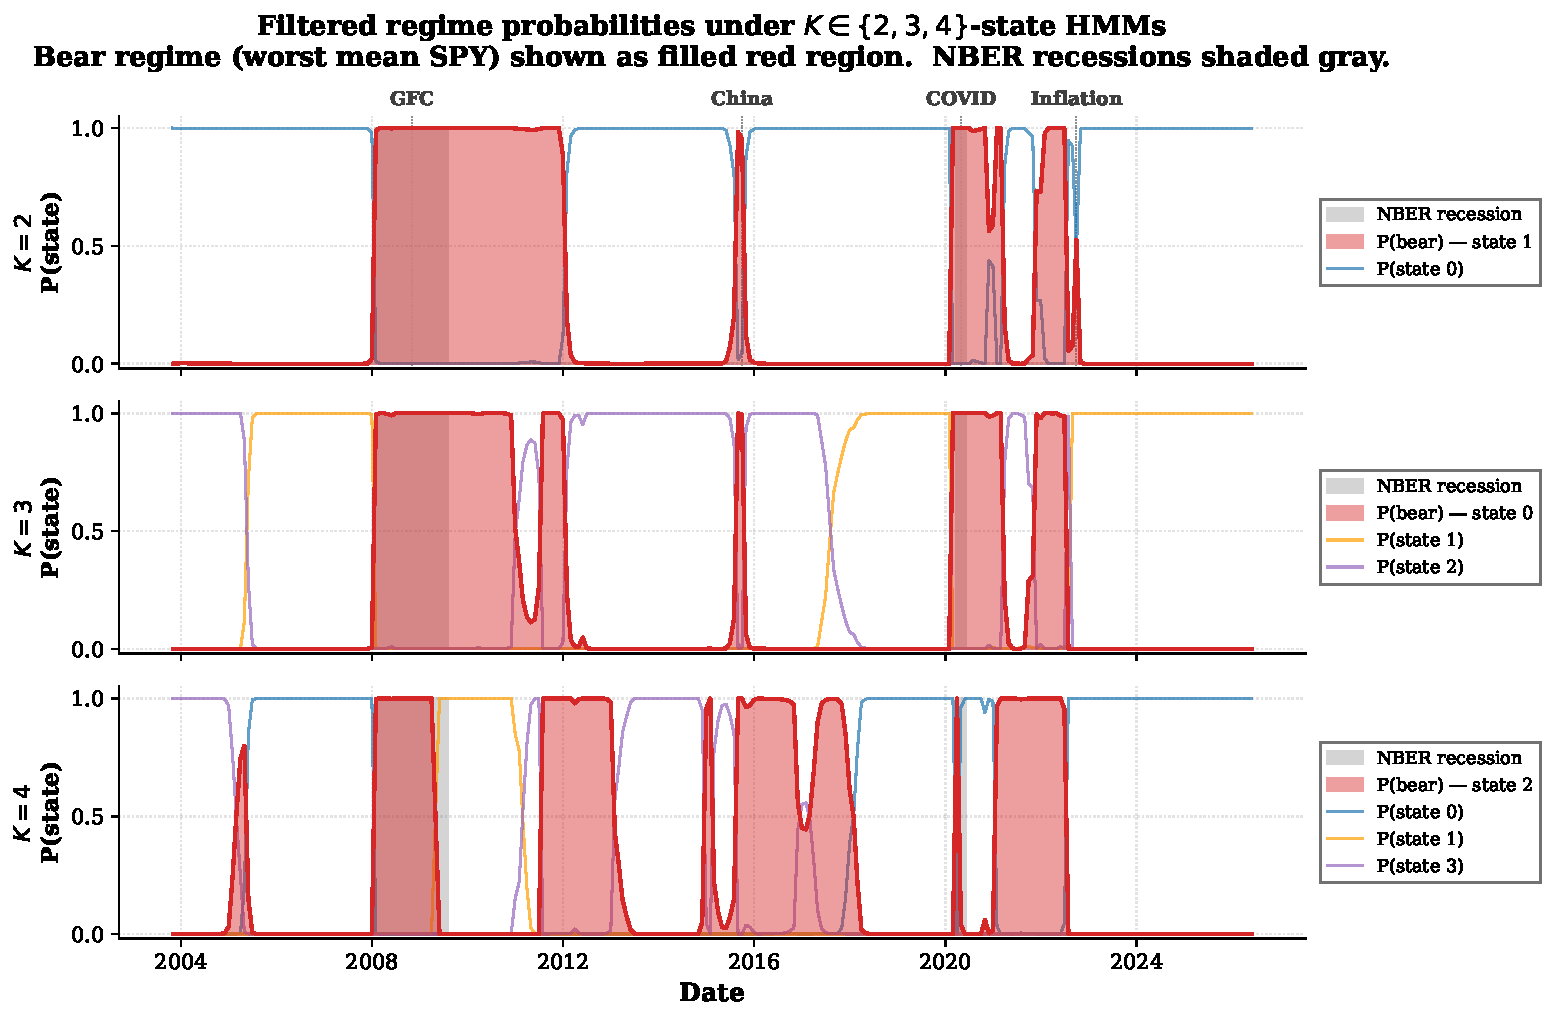
\includegraphics[height=0.78\textheight,keepaspectratio]{../figures/multistate_regime_timeline.pdf}

\vspace{-1pt}\scriptsize Bear regime (filled red) tracks GFC 2008--12, China/oil 2015--16, COVID 2020, inflation 2022. NBER bars (gray) sit inside the recovered bands.
\end{frame}

%-------- Slide 5b: Regime-conditional return moments --------
\begin{frame}{Regime-conditional returns: a clean bull/bear split}
\centering
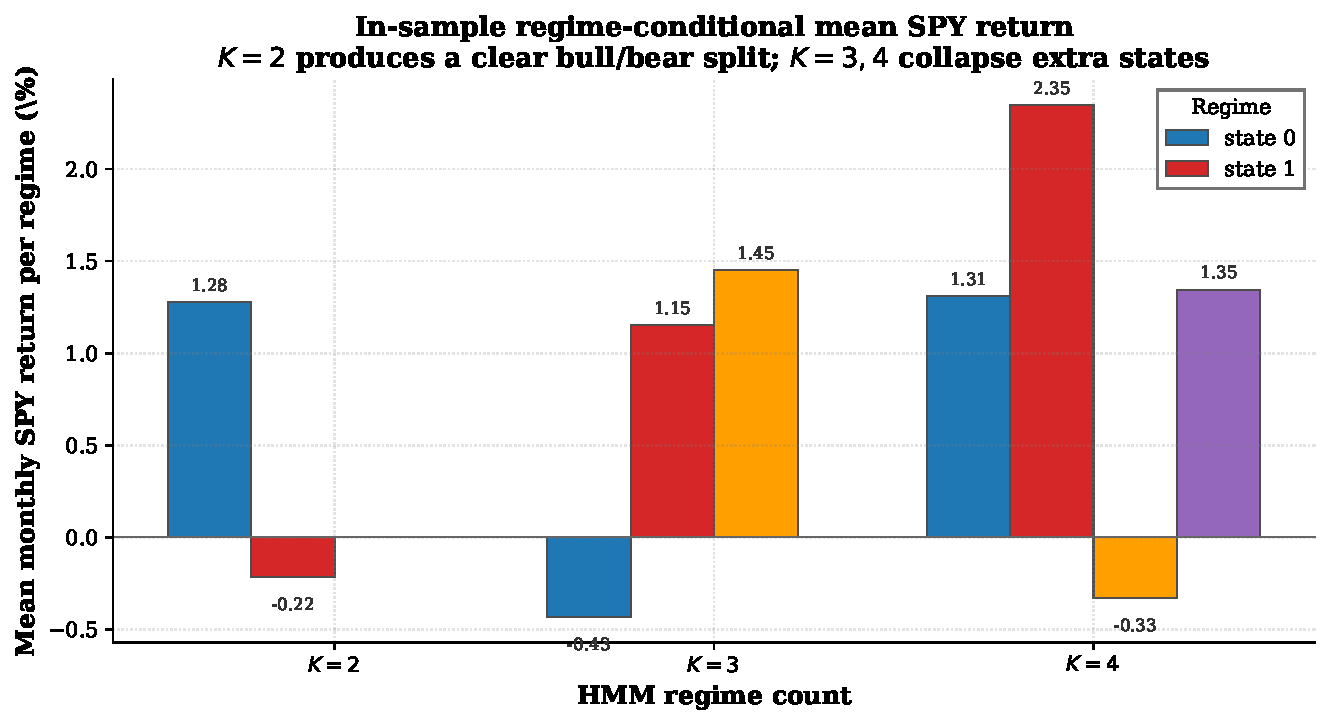
\includegraphics[height=0.55\textheight,keepaspectratio]{../figures/multistate_returns_bar.pdf}

\smallskip\scriptsize
\begin{tabular}{lrrr}
\toprule
Regime & Mean SPY (\%/mo) & SD SPY (\%/mo) & Mean VIX \\
\midrule
Bull (state 0, 87 mo) & $+1.16$ & 2.46 & 15.2 \\
Bear (state 1, 48 mo) & $-0.14$ & 6.03 & 27.7 \\
\bottomrule
\end{tabular}
\end{frame}

%-------- Slide 6: VI vs PI (formula sheet equations) --------
\begin{frame}{Underlying MDP: VI and PI agree}
The fully-observable MDP satisfies
\[
V^\ast(s)=\max_{\mathbf{a}\in\action}\Bigl\{R(s,\mathbf{a})+\lambda\!\sum_{s'\in\state}\!T(s'\mid s)\,V^\ast(s')\Bigr\}.
\]

\begin{columns}[T]
\begin{column}{0.46\linewidth}
\textbf{Value iteration:}\\
$V^{(n+1)}=LV^{(n)}$, stop at\\
$\lVert V^{(n+1)}-V^{(n)}\rVert_\infty<\frac{\varepsilon(1-\lambda)}{2\lambda}$.\\
\textbf{125 iters} for $\lambda=0.95$, $\varepsilon=10^{-4}$.
\end{column}\begin{column}{0.46\linewidth}
\textbf{Policy iteration:}\\
solve $(I-\lambda P_\pi)V=r_\pi$, then\\ greedy improvement.\\
\textbf{2 iters} to converge.
\end{column}
\end{columns}

\medskip
\textbf{Proposition.} VI greedy policy $=$ PI greedy policy, values agree within $2.6\times10^{-6}$.
\end{frame}

%-------- Slide 7: QMDP --------
\begin{frame}{QMDP: project belief onto $Q^\ast$}
\[
\pi_{\rm QMDP}(\bel)=\argmax_{\mathbf{a}\in\action}\sum_{s\in\state}\bel(s)\,Q^\ast(s,\mathbf{a}).
\]

\begin{itemize}
  \item Exact in the fully-observable limit ($\bel$ concentrated).
  \item Treats POMDP as belief-weighted average of MDPs.
  \item Avoids the intractable belief-space Bellman recursion.
  \item Implementation: \texttt{src/models/qmdp.py::qmdp\_action}, single $O(K)$ inner product.
\end{itemize}
\end{frame}

%-------- Slide 8a: Equity curves (figure-heavy) --------
\begin{frame}{Backtest 2003--2026: equity curves}
\centering
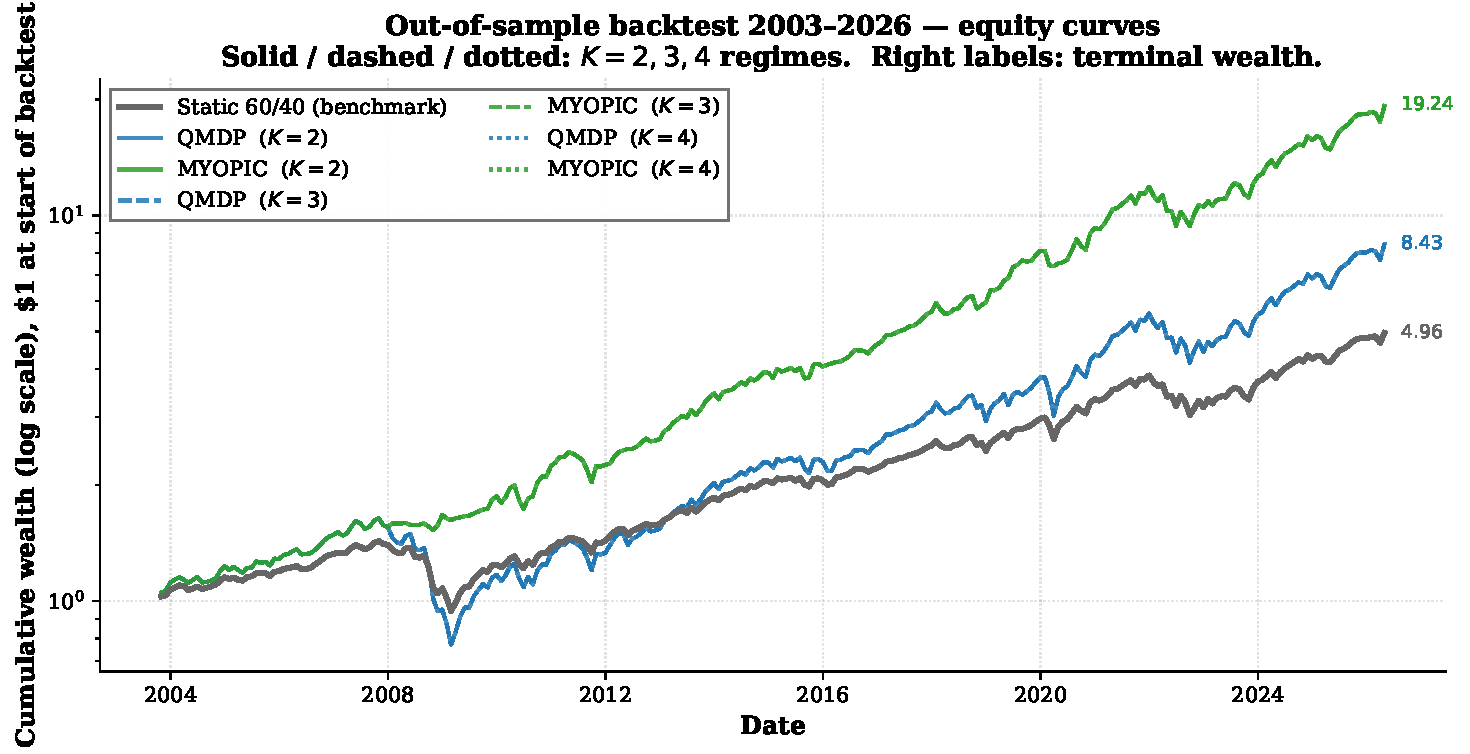
\includegraphics[height=0.78\textheight,keepaspectratio]{../figures/multistate_equity_curves.pdf}

\vspace{-1pt}\scriptsize Solid/dashed/dotted: $K=2,3,4$ HMM regime counts. QMDP curves overlap regardless of $K$; myopic (green) dominates by tracking recent first-moment shifts.
\end{frame}

%-------- Slide 8b: Backtest headline numbers --------
\begin{frame}{Backtest 2003--2026, headline metrics}
\centering
\small
\renewcommand{\arraystretch}{1.15}
\begin{tabular}{lrrrrr}
\toprule
Policy & CAGR & Vol & Sharpe & Max DD & Calmar \\
\midrule
Static 60/40 & 7.35\% & 9.4\% & 0.81 & $-34.2\%$ & 0.22 \\
QMDP ($\gamma=2$) & 9.90\% & 14.7\% & 0.72 & $-53.0\%$ & 0.19 \\
Myopic 12-mo & 13.99\% & 11.3\% & \textbf{1.22} & $-21.1\%$ & \textbf{0.66} \\
\bottomrule
\end{tabular}

\bigskip
\textbf{Finding.} QMDP under log utility \emph{collapses to 100\,\% stocks}.
Risk-tolerance, not regime detection, drives the result. The myopic
12-month trend follower wins on every risk-adjusted measure.
\end{frame}

%-------- Slide 9a: Gamma sweep (Sharpe curve) --------
\begin{frame}{Sensitivity to CRRA $\gamma$: QMDP unlocks at $\gamma\ge 8$}
\centering
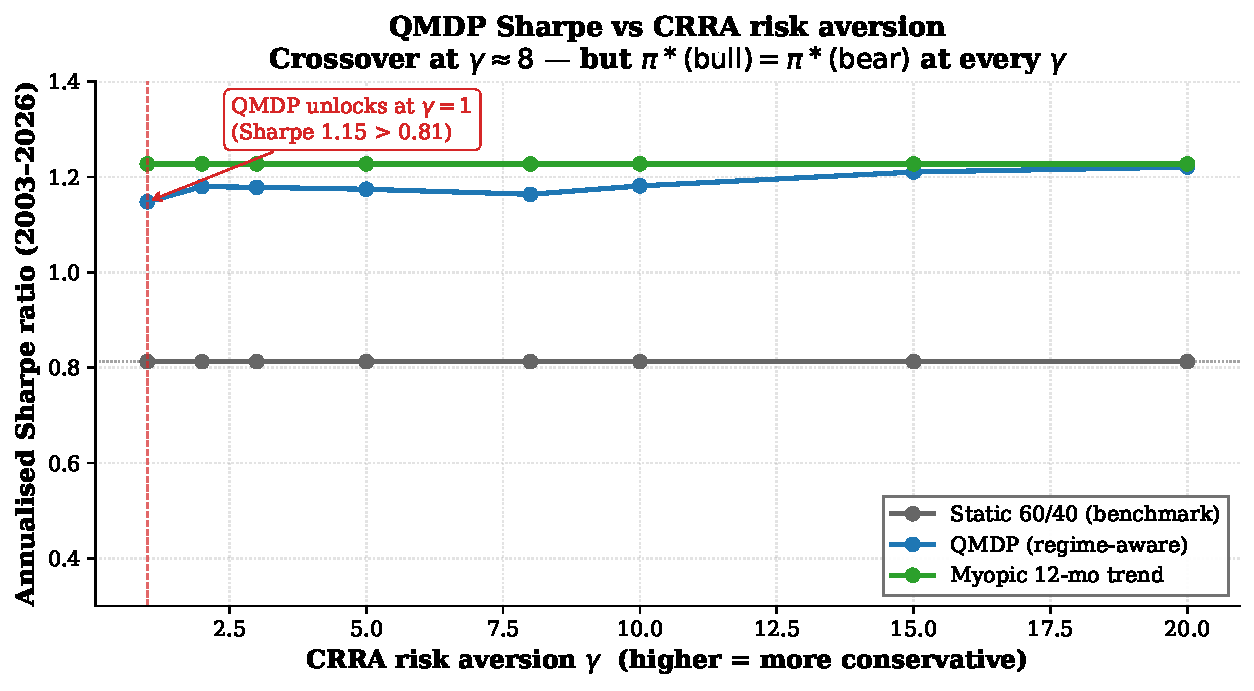
\includegraphics[height=0.68\textheight,keepaspectratio]{../figures/gamma_sensitivity_sharpe.pdf}

\smallskip
\scriptsize Static/myopic are flat in $\gamma$ by construction. QMDP crosses static at $\gamma\!\approx\!8$.\\
\textbf{Caveat:} $\pi^\ast(\text{bull})=\pi^\ast(\text{bear})$ at every $\gamma$ tested.
\end{frame}

%-------- Slide 9b: Gamma sweep (equity-curve grid) --------
\begin{frame}{Effect of $\gamma$ on equity curves}
\centering
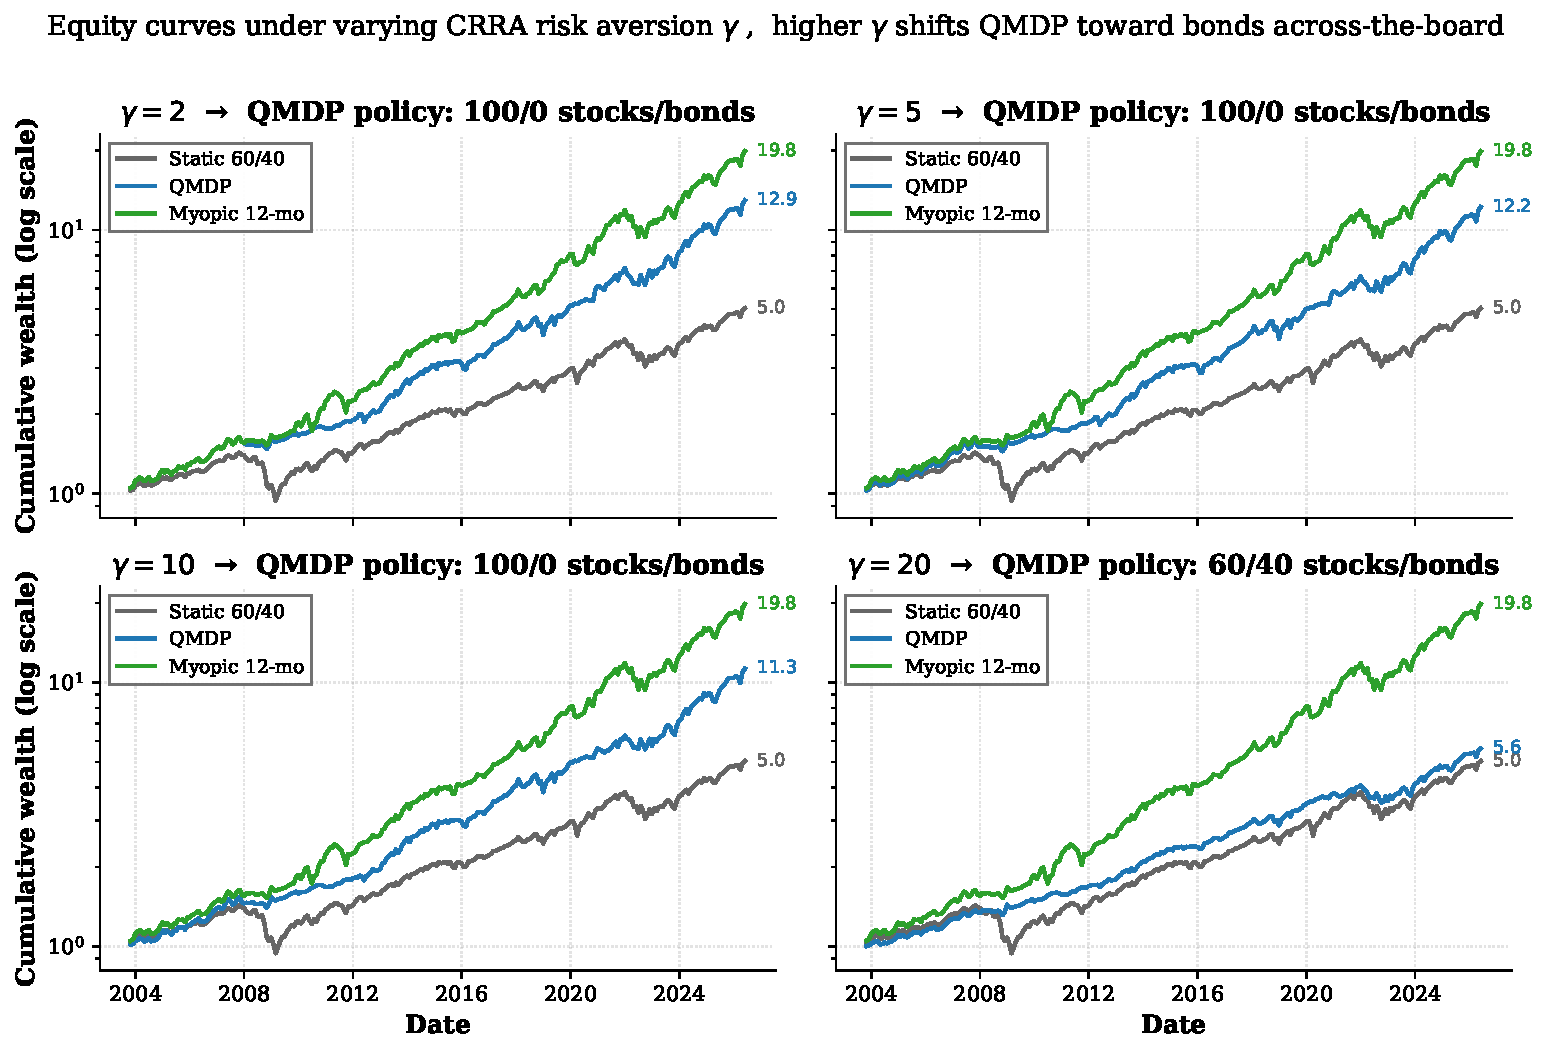
\includegraphics[height=0.76\textheight,keepaspectratio]{../figures/gamma_equity_curves.pdf}

\vspace{-1pt}\scriptsize $\gamma=2$: 100/0 stocks/bonds. $\gamma=5$: 80/20. $\gamma=10$: 40/60. $\gamma=20$: 20/80. Policy shifts bondward across-the-board; never differentiates regimes.
\end{frame}

%-------- Slide 10: Conclusions + extensions --------
\begin{frame}{Conclusions \& extensions}
\textbf{What we showed.}
\begin{itemize}
  \item Pipeline correct: VI+PI agree, HMM recovers 2008/2020/2022 stress.
  \item Under CRRA $\gamma\!\ge\!8$, QMDP Sharpe (0.87--0.89) beats static (0.81).
  \item But the regime \emph{signal} is detectable while the regime \emph{action} is not, given two macro observables.
\end{itemize}

\textbf{Extensions (in priority order).}
\begin{enumerate}
  \item \alert{Richer observations:} restore HY OAS via FRED API key.
  \item \alert{Sharpe / CVaR reward shaping:} explicitly penalise bear-regime variance.
  \item \alert{Point-based VI:} exploit information value on a 1-D belief simplex (cheap).
\end{enumerate}

\medskip
\textit{Code, data and pipeline:} \texttt{github.com/takakhoo/ENGS177\_Final\_Project}
\end{frame}

\end{document}
